\documentclass[12pt,a4paper]{report}
\usepackage[utf8]{inputenc}
\usepackage{graphicx}
% Para inclur las redes
\usepackage{tikz-network}
\usetikzlibrary{positioning}

\usepackage{caption}
\usepackage{listings}
\usepackage{xcolor}

\begin{document}

\begin{figure}
\center
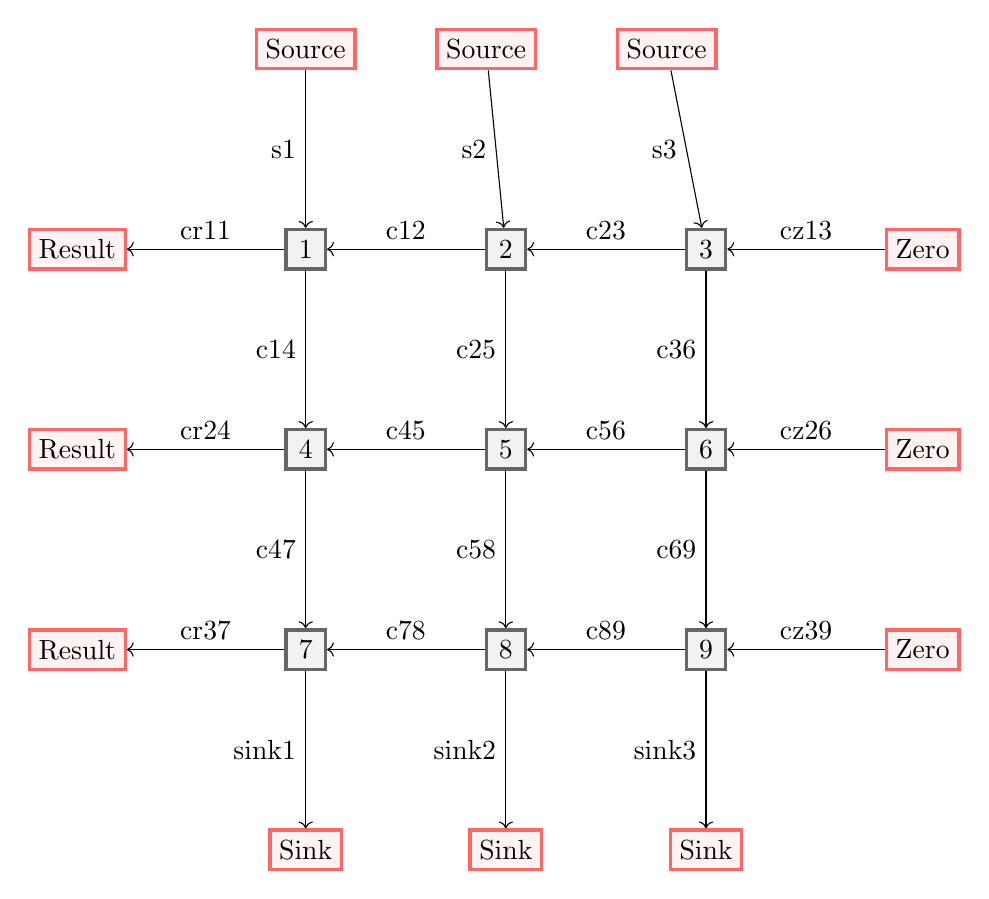
\begin{tikzpicture}[
squarednodered/.style={rectangle, draw=red!60, fill=red!5, very thick, minimum size=5mm},
squarednode/.style={rectangle, draw=black!60, fill=black!5, very thick, minimum size=5mm},
]
%Nodes
%%% Matriz interna 3X3
%%%% Primera fila
\node[squarednode]      (uno)       {1};
\node[squarednode]      (dos)       [right=2cm of uno] {2};
\node[squarednode]      (tres)       [right=2cm of dos] {3};

%%%% Segunda fila
\node[squarednode]      (cuatro)      [below=2cm of uno] {4};
\node[squarednode]      (cinco)       [below=2cm of dos] {5};
\node[squarednode]      (seis)       [below=2cm of tres] {6};

%%%% Tercera fila fila
\node[squarednode]      (siete)      [below=2cm of cuatro] {7};
\node[squarednode]      (ocho)       [below=2cm of cinco] {8};
\node[squarednode]      (nueve)       [below=2cm of seis] {9};

%%% Nodos source
\node[squarednodered]   (sourceUno) [above=2cm of uno]{Source};
\node[squarednodered]   (sourceDos) [right=1cm of sourceUno]{Source};
\node[squarednodered]   (sourceTres) [right=1cm of sourceDos]{Source};

%%% Nodos Zero
\node[squarednodered]   (zeroUno) [right=2cm of tres]{Zero};
\node[squarednodered]   (zeroDos) [right=2cm of seis]{Zero};
\node[squarednodered]   (zeroTres) [right=2cm of nueve]{Zero};

%%% Nodos Result
\node[squarednodered]   (resultUno) [left=2cm of uno]{Result};
\node[squarednodered]   (resultDos) [left=2cm of cuatro]{Result};
\node[squarednodered]   (resultTres) [left=2cm of siete]{Result};

%%% Nodos Sink
\node[squarednodered]   (sinkUno) [below=2cm of siete]{Sink};
\node[squarednodered]   (sinkDos) [below=2cm of ocho]{Sink};
\node[squarednodered]   (sinkTres) [below=2cm of nueve]{Sink};


%Lines
%%% Matriz interna
%%%% Horizontales
\draw[->] (tres) --  (dos) node[midway,above] {c23};
\draw[->] (dos) -- (uno)node[midway,above] {c12};
\draw[->] (cinco) --  (cuatro) node[midway,above] {c45};
\draw[->] (seis) -- (cinco)node[midway,above] {c56};
\draw[->] (ocho) --  (siete) node[midway,above] {c78};
\draw[->] (nueve) -- (ocho)node[midway,above] {c89};

\draw[->] (zeroUno) --  (tres) node[midway,above] {cz13};
\draw[->] (zeroDos) --  (seis) node[midway,above] {cz26};
\draw[->] (zeroTres) --  (nueve) node[midway,above] {cz39};

\draw[->] (uno) --  (resultUno) node[midway,above] {cr11};
\draw[->] (cuatro) --  (resultDos) node[midway,above] {cr24};
\draw[->] (siete) --  (resultTres) node[midway,above] {cr37};

%%%% Verticales
\draw[->] (uno) --  (cuatro) node[midway,left] {c14};
\draw[->] (cuatro) --  (siete) node[midway,left] {c47};
\draw[->] (dos) --  (cinco) node[midway,left] {c25};
\draw[->] (cinco) --  (ocho) node[midway,left] {c58};
\draw[->] (tres) --  (seis) node[midway,left] {c36};
\draw[->] (seis) --  (nueve) node[midway,left] {c69};

%%% Sources
\draw[->] (sourceUno) --  (uno) node[midway,left] {s1};
\draw[->] (sourceDos) --  (dos) node[midway,left] {s2};
\draw[->] (sourceTres) --  (tres) node[midway,left] {s3};

%%% Sink
\draw[->] (siete) --  (sinkUno) node[midway,left] {sink1};
\draw[->] (ocho) --  (sinkDos) node[midway,left] {sink2};
\draw[->] (nueve) --  (sinkTres) node[midway,left] {sink3};


\end{tikzpicture}
\end{figure}

\pagebreak

\begin{gather}
 \begin{bmatrix} 1 & 2 & 3 \\ 
 4 & 5 & 6 \\
  7 & 8 & 9 \end{bmatrix}
 \times
  \begin{bmatrix}
  	1 & 0& 2\\
  	0 & 1 & 2\\
  	1 & 0 & 0   \end{bmatrix}
  	=
  	  \begin{bmatrix}
  	4 & 2 & 6\\
  	10 & 5 & 18\\
  	16 & 8 & 30   \end{bmatrix}
\end{gather}
\end{document}